\section{Data} \label{sec:data}

The data used in this work were obtained using the Bench for Optical Testing (BOT), which was built and designed at SLAC National Accelerator Laboratory. BOT allows laboratory tests with the LSSTCam with variations of less than 5 \% in flat images so that measurements of the linearity, full well, and gain of the PTCs can be made \citep{newbry2018lsst}. Figure \ref{fig:BOT_stand} shows the structure of the BOT, where the cryostat is located in the circular top and the focal plane is pointing down the test bench. 

%Los datos utilizados en este trabajo fueron obtenidos mediante el banco de pruebas Bench for Optical Testing (BOT), que fue construido  y diseñado en SLAC National Accelerator Laboratory, el cual permite realizar pruebas de laboratorio con la LSSTCam con variaciones menores a 5\% en imágenes flat de modo que puedan efectuarse medidas de la linealidad, full well y la ganancia de las PTC \citep{newbry2018lsst}. En la figura \ref{fig:BOT_stand} se muestra la estructura del BOT, donde en la parte superior circular va el criostato y el plano focal queda apuntando hacía abajo del banco de pruebas. 


\begin{figure}[!htb]
    \centering
    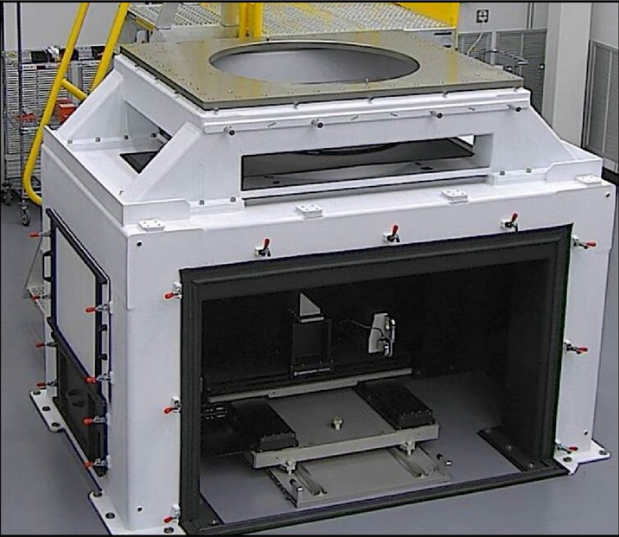
\includegraphics[width=0.7\textwidth]{Figures/BOT_stand.png}
    \caption{Bench for Optical Testing (BOT) designed by SLAC. Figure is taken from \cite{newbry2018lsst}. }
    \label{fig:BOT_stand}
\end{figure}

The \textit{run 13144} and \textit{run 13186} were used, the latter containing the crosstalk matrix information. According to \cite{snyder2020laboratory}, the electronic crosstalk measurements are carried out using a projector called \textit{crosstalk projector}, which illuminates a single sensor with a pattern of large bright spots with a collimated beam of light, which has a radius of 80 pixels. However, to perform laboratory tests simulating real source sizes they used the optical projector called \textit{the spot grid projector}. This projector generates spots in specific grids and has filters that simulate both lines left by satellites and the signal level of the sky background.

%Se hizo uso de los \textit{run 13144} y \textit{run 13186}, siendo este último el que contiene la información de la matriz de crosstalk. De acuerdo con \cite{snyder2020laboratory} las mediciones del crosstalk electrónico es llevado a cabo mediante un proyector llamado \textit{proyector crosstalk}, el cual ilumina un solo sensor con un patrón de grandes puntos brillantes con un haz de luz colimado, que posee un radio de 80 pixeles. Sin embargo, para hacer las pruebas de laboratorio simulando tamaños de fuentes reales se utiliza el proyector óptico llamado \textit{the spot grid projector}, que genera puntos en grids específicos y cuenta con filtros que simulan tanto líneas dejadas por satélites, como el nivel de señal del fondo del cielo.